\documentclass[accentcolor=tud1c,colorback,ngerman,12pt] {tudreport}
\usepackage[utf8]{inputenc}
\usepackage{babel}
\usepackage{acronym}
\usepackage{listings}
\usepackage{tabularx}
\usepackage{url}
\usepackage{hyperref}

\lstset{language=C,basicstyle=\small, breaklines=true, showtabs=false, showspaces=false, showstringspaces=false}

\renewcommand{\lstlistingname}{Quelltext}
\lstset{literate=%
{Ö}{{\"O}}1
{Ä}{{\"A}}1
{Ü}{{\"U}}1
{ß}{{\ss}}1
{ü}{{\"u}}1
{ä}{{\"a}}1
{ö}{{\"o}}1
}

\setinstitutionlogo[height]{bilder/rechnersysteme-transparent}

\begin{document}
\title{Implementierung eines multithreaded TCP/IP Stacks für einen auf AMIDAR basierten Java Prozessor}
\subtitle{Bachelorarbeit}
\subsubtitle{Robert Wiesner \hfill  \\31. Mai 2017}

\maketitle
\chapter*{Erklärung gemäß § 22 Abs. 7 APB}

Hiermit erkläre ich gemäß § 22 Abs. 7 der Allgemeinen Prüfungsbestimmungen (APB) der Technischen Universität Darmstadt in der Fassung der 4. Novelle vom 18. Juli 2012, dass ich die Arbeit selbstständig verfasst und alle genutzten Quellen angegeben habe und bestätige die Übereinstimmung von schriftlicher und elektronischer Fassung.\\ \\ \\ \\

\parbox{8cm}{\centering Darmstadt, den 31. Mai 2017\hrule
\strut \centering\footnotesize Ort, Datum} \hfill\parbox{8cm}{\phantom{Darmstadt, den 31. Mai 2017} \hrule
\strut \centering\footnotesize Robert Wiesner}

\vfill

\noindent \textbf{Fachbereich Elektro- und Informationstechnik}\\
Institut für Datentechnik\\
Fachgebiet Rechnersysteme\\
Prüfer: Prof. Dr.-Ing. Christian Hochberger\\
Betreuer: Dipl.-Inform. Changgong Li

\tableofcontents

\chapter{Einleitung}

AMIDAR, steht für Adaptive Microinstruction Driven Architecture, dabei handelt es sich um ein Modell eines adaptiven Prozessors, das es diesem erlaubt zur Laufzeit einer Anwendung auf deren spezifische Anforderungen zu reagieren. Dazu gehört das Anpassen von Busstrukturen und bestehenden Funktionseinheiten, sowie die Synthese von neuen Funktionseinheiten.
Im Fachgebiet Rechnersysteme der TU-Darmstadt wird momentan ein Prototyp in Form eines Java-Prozessors implementiert. \\\\
Dieser wird zur Zeit erweitert, mit dem Ziel die Performance deutlich zu erhöhen. Um die Verbesserung der Laufzeit zu evaluieren fehlen Beispielanwendungen. Eine wichtige Anwendung im Umfeld von eingebetteten Systemen ist der TCP/IP Stack.\\\\
Zum Zeitpunkt der Arbeit verfügt AMIDAR mit der dazugehörigen API bereits über grundlegende Netzwerk-Funktionalitäten. Dazu gehören die Unterstützung für die Protokolle Ethernet, ARP, begrenzt IPv4 und UDP. Mit UDP kann keine verlustfreie Datenübertragung garantiert werden, welche für viele Netzwerkanwendungen vorausgesetzt wird.\\\\
Im Rahmen dieser Arbeit wurde ein TCP-Stack entwickelt, sowie der IP-Stack erweitert um eine geordnete und verlustfreie Datenübertragung zu realisieren. Die Funktionalität von diesem wurde mit einen auf einem FPGA synthetisierten AMIDAR System getestet.

\chapter{Implementierung}
Im Rahmen dieser Arbeit wurde ein TCP Stack für die API des AMIDAR Microprozessor entwickelt. Darüber hinaus wurde 

\section{Überblick}
Vor Beginn dieses Projekts verfügte die AMIDAR Java API über Grundlegende Netzwerk Funktionen. Dazu gehört der Netzwerktreiber, ein IP-Stack mit ARP Funktionalität und ein UDP Stack. Neu geschrieben wurde im Rahmen dieses Projekts der Multithreading Fähige TCP Stack. Dieser wurde in die vorhandene Software Integriert. Desweiteren wurde der IP-Stack erweitert und optimiert. \\
Sowohl beim Senden als auch beim Empfangen von Datenpaketen greifen die einzelnen Module in einander über. Zum empfangen von Daten Prüft der Prozess des Netzwerktreibers ob neue Ethernet Frames vorliegen. Wenn das der Fall wird, eine Funktion im IP Stack aufgerufen, die die Ethernet Frames überprüft. Der IP-Stack unterscheidet die Pakete zwischen ARP und IP. ARP anfrage werden geprüft und gegebenenfalls beantwortet. Handelt es sich bei den Datagramm um ein IP-Paket, wird ein entsprechendes Objekt erzeugt und nach weiterer Überprüfung entweder an den UDP-Stack oder an den TCP-Stack übergeben. Die Stacks für TCP und UDP beinhalten jeweils einen Table mit den vorhandenen Verbindungen, die durch Ziel und Quell Port identifiziert werden können. Ihnen können gegebenenfalls die Erzeugten Pakete weiter gegeben werden, wo sie zwischengespeichert werden. Im Falle von UDP wird von den dieses die Payload ausgelesen, wenn auf "receive"{} Methode der UDP-Connection, von einen anderen Thread aufgerufen wird. Die TCP-Connections können jeweils in ihren eigenen Thread laufen, da eine Zeitnahe Verarbeitung der angekommen Pakete nötig ist um die Verbindung zu managen. In diesem Thread werden die angekommenen Pakete ausgewertet und die dazu entsprechenden Reaktionen berechnet und ausgeführt. \\
Wenn UDP Datenpakete versendet werden sollen, wird die {}"Send"{} Methode aufgerufen, die ein UDP-Paket erzeugt und diesen an den UDP-Stack weitergibt. Der wiederum ruft den erzeugt aus dem UDP-Paket ein IP-Paket. Mit dem die {}"Send"{} Methode des IP-Stacks aufgerufen wird. Die letztendlich einen Ethernetframe erzeugt und mit den EthernetWrapper den Sendevorgang startet.\\ 
Bei dem senden von Daten über TCP wird von der Anwendung der ebenfalls die {}"Send"{} Methode der TCP-Connection aufgerufen. Die werden dabei jedoch nicht sofort gesendet, sondern in einen Puffer zwischengespeichert, vorausgesetzt der aktuelle Status der Verbindung erlaubt das. Bei Ausführung des Threads der Verbindung, werden gegebenenfalls die zu übertragenden TCP-Pakete in IP Pakete umgewandelt und analog wie die UDP-Pakete versendet. 



\section{IP Stack}
Der IP Stack erfüllt mehrere Funktionen, die für eine zuverlässige Netzwerkkommunikation benötigt werden. Dazu gehört, das Senden und Empfangen von IP-Pakten, als auch die Unterstützung der ARP Funktionalitäten.

\subsection{Empfangen von IP Paketen}

Die Methode readIpPakets() des IP-Stacks, die vom Netzwerktreiber Thread aufgerufen. In dieser werden in einer Schleife die angekommenen Ethernet Pakete eingelesen und die IP Pakete dazu erzeugt. Dabei werden im Zweifelsfall Fragmente von fragmentierten Paketen zwischengespeichert, bis diese vollständig sind. \\
Bei den so erzeugten IP-Paketen wird das darüber liegende Protokoll ausgelesen.\\
Damit UDP und TCP Pakete zugestellt werden können müssen die jeweiligen Stacks im IP-Stack registriert werden. Nach der Registrierung können angekommene  Pakete den jeweiligen Stack zugeordnet werden. Dafür implementieren beide Stacks die Function "notificateByIpStack()" der eine Liste mit angekommenen UDP-Paketen übergeben wird. 

\subsubsection{Fragmentierung}

IP Pakete können während der Übertragung fragmentiert werden. Um über Netzwerke mit einer zu niedrigen Maximalen Segment Größe übertragen zu werden. Diese werden vom Empfänger defragmentiert. \\
Fragmentierte Pakete können nach der dem erzeugen erkannt werden, in dem das entsprechende Flag ausgelesen wird. Die Flag gibt nicht explizit an, das diesen Paket Teil eines größeren fragmentierten Pakets ist, sondern dass sie ein Teil eines fragmentierten Pakets sind und weitere Pakete Fragmente folgen. Das bedeutet, dass das letzte Fragment eines Pakets nicht das Flag gesetzt hat, dieses kann man daran erkennen, dass der Fragment Offset ungleich Null ist\\
Der IP Stack enthält eine Liste von für Fragmentierte Pakete, die Listen mit jeweils zusammengehörigen Fragmenten enthält. Wannn immer ein Paket ankommt, bei dem die {}"More Fragments"{} Flag gesetzt ist oder die Data Offset ungleich Null ist, wird geprüft, ob dieses zu einem der fragmentierten Pakete gehört, und wird in diesem Fall an eine der Listen hinzugefügt. Die Zugehörigkeit wird dabei anhand der Identification des IP Pakets geprüft. \\
Falls ein Paket ohne Flag einen anderen Fragmentierten Paket zugeordnet werden kann, ist dieses das letzte Fragment des ursprünglichen IP Pakets, mit dem das kombinierte Paket erzeugt werden kann. \\
Für diesen Zweck verfügt die Klasse IpPaket über die statische Methode "{}fuseFragmentedIpPackets()"{}, die eine Liste von zusammengehörigen IP-Paket Fragmenten annimmt. Diese werden auf Kompatibilität geprüft, wobei auch die Größe der kombinierten Nutzlast berechnet wird. Die Fragmente müssen neben der identischen Identifikation über die selbe Quell und Ziel IP-Adresse verfügen. Des weiteren müssen die Angaben des Frame Offsets mit der Paketlänge Plausibel sein. \\
Anschließend werden die Pakete wird ein Array der entsprechenden Länge erzeugt und die Nutzlast der Pakete anhand des Frame Offsets zusammengesetzt. Danach kann der Konstruktor der IP-Paket Klasse aufgerufen werden, wobei ihm die neu kombinierte Nutzlast übergeben wird.  Das neu erzeugte Paket wird zurückgegeben und von dem IP-Stack weiter verarbeitet. 


\subsection{Senden von IP Paketen}
Der IP-Stack verfügt über die Methode "sendIpPaket", die im Normalfall von dem TCP- oder dem UDP-Stack aufgerufen wird. Diese nimmt ein übergebenes IP-Paket an und generiert daraus einen Ethernet Frame. Daraufhin wird das Packet über Ethernet versendet. 


\subsection{Address Resolution Protokoll (ARP)}
Das ARP Protokoll wird verwendet um in einen lokalen Netzwerk die IP Adressen zu den physischen MAC-Adressen aufzulösen. Ein Host, kann einer ARP-Request als Broadcast verschicken um die MAC-Adresse zu erfahren, über die der die Netzwerkressource mit der IP-Adresse zu erreichen ist. 

Der IP-Stack verfügt über die Möglichkeit ankommende ARP Pakte zu verarbeiten. Für den Fall, das es sich bei einen ankommenden Datenpaket anstatt eines IP-Pakets um ein ARP-Paket handelt, wird geprüft, ob es sich um eine {}"Request"{} oder eine {}"Response"{} handelt. Für den Fall, das es sich um eine Request handelt, wird in einer entsprechenden Antwort die eigene physische MAC Adresse verschickt. 






\section{TCP Stack}

\section{Zero Copy}
Die TCP und IP Pakete werden jeweils durch eine entsprechende Klasse repräsentiert. Die Objekte dieser Klasse enthalten jeweils ein Array, dass Header und Nutzdaten des Pakets enthält. Beide Klassen verfügen über einen Konstruktor, der jeweils die andere der beiden Klassen als Parameter entgegen nimmt. So kann beim Senden aus einen TCP-Paket ein IP-Paket erzeugt werden und beim Empfangen aus einen IP-Paket ein TCP-Paket erzeugt werden. Dabei stellt das TCP-Paket die Nutzlast des IP-Pakets da. Um in diesen Fall lange Kopiervorgänge zu ersparen wird es vermieden ein neues Array anzulegen und die Daten rein zu kopieren. Anstelle dessen wird in der TCP-Paket Klasse im Array ein 20 Byte Puffer eingeplant, in dem der IP-Header später geschrieben werden kann. Bei der Erzeugung eines IP-Pakets aus einen TCP-Paket wird das im TCP-Paket erzeugte Array weiterverwenden und da die ersten 20 Byte leer sind, kann dort der IP Header geschrieben werden. 


\section{DHCP}

\section{Stream Sockets}


\chapter{Evaluation}


\section{Testaufbau}

Zur Evaluation wurde ein Nexys-Video-FPGA-Entwickler-Board verwendet. Auf diesem wurde Java-Prozessor der AMIDAR-Klasse synthetisiert. Als Netzwerkschnittstelle wurde eine Steckkarte mit zwei Ethernet RJ45 Schnittstellen verwendet. Diese wurde mit einem Patch-Kabel zu der Ethernet Schnittstelle eines Laptops verbunden. Der Laptop verfügt über eine Realtec Gigabit Ethernet Schnittstelle. Des Weiteren läuft auf dem Laptop Ubuntu 16.04 und ein "{}ISC-DHCPD"{} DHCP-Server. Für Testzwecke wurden außerdem diverse Java-Programme genutzt, welche die Java-Netzwerksockel nutzen. 

\subsection{Konfiguration des verwendeten AMIDAR-Systems}
Für die Evaluation wurde ein System mit einer Taktrate von 100MHz verwendet. Dieses entspricht zum dem Zeitpunkt der Abgabe der neusten verfügbaren Konfiguration. Einschließlich des neuen Bus-Systems und Heaps, der über einen deutlich schnelleren Cache verfügt, als die ältere Variante. \\
Ein Nachteil dieser Konfiguration ist, dass ein Scheduler mit reduzierter Funktionalität verwendet wurde, da der alte Scheduler Fehler enthielt, mit denen ein Multithreading fähiger TCP-Stack nicht hätte umgesetzt werden können und der neue Hardware-Scheduler noch nicht einsatzbereit war. Aus diesen Grund könnten sich die hier gemessen Testergebnisse deutlich verbessern, sobald der neue Scheduler eingebaut ist. \\
Des Weiteren wurde zu diesem System über den AMIDAR-Systembuilder ein Ethernet-Controller hinzugefügt, mit dem die angeschlossene Netzwerk-Platine genutzt werden kann.


\begin{figure}
	\centering
	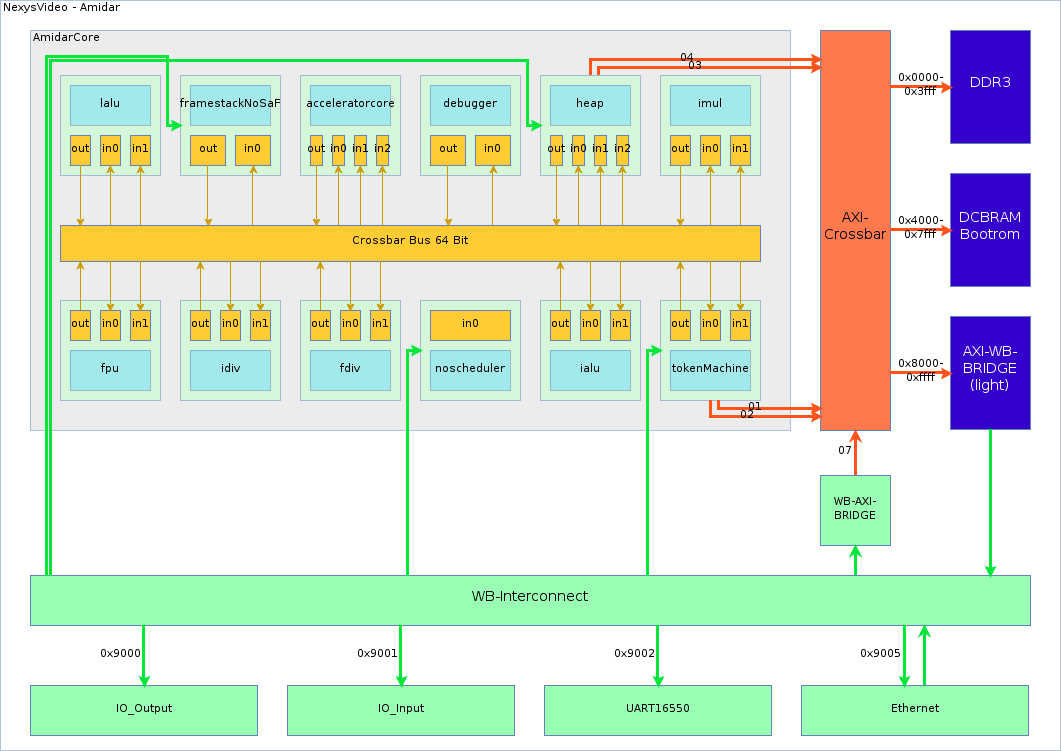
\includegraphics[width = 1\textwidth]{Graphics/system.png}
	\caption{Konfiguration des verwendeten AMIDAR-Systems, automatisch generiert durch den AMIDAR-Systembuilder}

\end{figure}

\FloatBarrier
\section{Grundlegende Funktionen}

Für das Testen der Grundfunktionen wurden mehrere Testszenarien verwendet. Zum einen wurde ein einfacher Echo-Server auf AMIDAR laufen gelassen, der ankommende Wörter zurücksendet. Dieser wurde auf einem oder mehreren Threads aufgeführt. Eine auf dem Laptop laufende Java-Anwendung sendet dabei eingegebene Textnachrichten und wartet auf die Antwort des Servers, welche in der Konsole ausgegeben wird. Dabei wird sowohl der Verbindungsaufbau als auch das Empfangen und Senden von Nachrichten getestet. Dies funktioniert auch mit mehreren offenen Verbindungen parallel. \\\\
Eine Anfrage bei einem DHCP Server funktioniert ebenfalls problemlos, wie sich dem Wireshark Screenshot im Anhang entnehmen lässt. \autoref{DHCP}




\section{Leistung}
Für die Leistungsmessung wird eine Mischung von Daten verwendet, die entweder mit Wireshark ausgelesen wurden, in den Testanwendungen auf dem Laptop in eine .csv Datei geloggt, oder während dem Betrieb auf AMIDAR ermittelt und über UART ausgegeben wurden. 
Die Latenz der einzelnen Pakete wurde Wireshark entnommen. Da Wireshark auf dem Laptop lief, ist die Übertragungszeit des letzten Pakets, das vom Laptop in einem Handshake gesendet wurde nicht gemessen worden. \\
Beim drei Wege Handshake, der von dem Laptop initiiert wurde, betrug die RTT nach dem Senden des SYN-Paketes bis zum Eintreffen des SYN-ACK-Pakets 15-30 Millisekunden. Momentan gibt es eine recht große Schwankung der Reaktionszeit. 

Falls die Übertragung von AMIDAR initiiert wird, benötigt der Laptop 900 Millisekunden, um auf die Anfrage zu reagieren. Nach weiteren 40 Millisekunden trifft das ACK-Paket von AMIDAR ein.\\\\
In einem weiteren Test wurden zehn Verbindungen zum selben Zeitpunkt geöffnet, über die jeweils in kurzen Abständen 500 Byte an Daten übertragen wurden. Diese Daten wurden von AMIDAR als Echo zurückgesendet. Dieses Szenario soll einen Server-Betrieb simulieren, bei dem Anfragen mehrerer Clients beantwortet werden sollen. Die Latenz dieser Übertragung wurde in einer Logdatei gespeichert und betrug zwischen 1,4 und 3,5 Sekunden. Dabei entfiel der größte Teil der Zeit auf das Auslesen der Daten aus den ankommenden Datenpaketen.\autoref{Multithread}\\

\begin{tabular}{cccc}
\# & Start Time$[ms]$ & End Time $[ms]$ & Response Time$[ms]$\\
1 &1495793145037&	1495793148691&	3654\\
2 &1495793149191&	1495793151370&	2179\\
3 &1495793151871&	1495793153906&	2035\\
4 &1495793154406&	1495793156688&	2282\\
5 &1495793157188&	1495793158886&	1698\\
6 &1495793159387&	1495793160988&	1601\\
7 &1495793161489&	1495793163013&	1524\\
8 &1495793163513&	1495793164989&	1476\\
\end{tabular}\\\\
Auffällig dabei ist, dass die Reaktionszeiten der einzelnen Verbindung mit weiteren Iterationen besser werden. \\
Bei diesem Testszenario wurden mit dem Statistik-Modul der AMIDAR-IDE folgende Werte ermittelt:\\\\
\begin{tabular}{lc}
jumpBytecodes & 16842753\\
total & 545259268 \\
distributedToken & 2004025412 \\
axi.transaction& 1\\
cache.hit & 65793\\
cache.hitrate& 0.996109\\
cache.miss& 257\\
outputFifoEmptyAtferFirstTransaction&16780707
\end{tabular}\\\\
Ein Problem, das bei diesem Versuch sichtbar wurde, ist die schwankende Latenz. Die Dauer eines Timeouts wird bei TCP relativ zur RTT bestimmt. Nach dem schnellen SYN-ACK mit kleinen Paketen wird im PC ein entsprechend kurzes Zeitlimit für Timeouts gesetzt. Das hat zur Folge, dass es zu Neuübertragungen größerer Datenpakete kommen kann, wenn diese auf der Seite des AMIDAR-Prozessors verarbeitet werden müssen, obwohl sie nicht verloren gegangen sind. \autoref{ret} \\\\
Die Übertragungsrate beim Senden wurde ermittelt, in dem ein zufällig generiertes Datenpaket in einer Schleife gesendet wurde. Dabei wird eine Übertragungsrate von 1333 kBit/s erreicht. Die Größe der einzelnen Datenpakete hat dabei nur einen vernachlässigbaren Einfluss auf die Nettoübertragungsrate, was darauf schließen lässt, dass das Bottleneck bei dem Sendepuffer liegt. \\\\
Dabei wurden mit dem Statistik-Modul des Debuggers folgende Werte ermittelt:\\\\
\begin{tabular}{lc}
jumpBytecodes & 537919489\\
total & 545259268 \\
distributedToken & 393412689 \\
axi.transaction& 1\\
cache.hit & 65793\\
cache.hitrate& 0.9960939\\
cache.miss& 258\\
outputFifoEmptyAtferFirstTransaction & 16781085
\end{tabular}






 

 
\chapter{Zusammenfassung}


\section{Fazit}

\section{Ausblick}

\section*{Abkürzungsverzeichnis}
\begin{acronym}
 \acro{CLB}{Configurable Logic Block}
 \acro{CPU}{central processing unit}
 \acro{ELF}{Executable and Linking Format}
 \acro{FPGA}{Field Programmable Gate Array}
 \acro{MC}{Microcontroller}
 \acro{CPU}{central processing unit}
 \acro{NCD}{Native Circuit Description Format}
 \acro{SoC}{System on Chip}
 \acro{Sph}{SpartanMC Hex Dateiformat}
 \acro{XDL}{Xilinx Design Language Format}




\end{acronym}

\listoffigures

\makeatletter
\renewcommand\chapter{\thispagestyle{\chapterpagestyle}%
                    \global\@topnum\z@
                    \@afterindentfalse
                    \secdef\@chapter\@schapter}
\makeatother

\nocite{*}
\bibliographystyle{alphadin}
\bibliography{Literaturverzeichnis}

\end{document}